% This is "sig-alternate.tex" V2.1 April 2013
% This file should be compiled with V2.5 of "sig-alternate.cls" May 2012
%
% This example file demonstrates the use of the 'sig-alternate.cls'
% V2.5 LaTeX2e document class file. It is for those submitting
% articles to ACM Conference Proceedings WHO DO NOT WISH TO
% STRICTLY ADHERE TO THE SIGS (PUBS-BOARD-ENDORSED) STYLE.
% The 'sig-alternate.cls' file will produce a similar-looking,
% albeit, 'tighter' paper resulting in, invariably, fewer pages.
%
% ----------------------------------------------------------------------------------------------------------------
% This .tex file (and associated .cls V2.5) produces:
%       1) The Permission Statement
%       2) The Conference (location) Info information
%       3) The Copyright Line with ACM data
%       4) NO page numbers
%
% as against the acm_proc_article-sp.cls file which
% DOES NOT produce 1) thru' 3) above.
%
% Using 'sig-alternate.cls' you have control, however, from within
% the source .tex file, over both the CopyrightYear
% (defaulted to 200X) and the ACM Copyright Data
% (defaulted to X-XXXXX-XX-X/XX/XX).
% e.g.
% \CopyrightYear{2007} will cause 2007 to appear in the copyright line.
% \crdata{0-12345-67-8/90/12} will cause 0-12345-67-8/90/12 to appear in the copyright line.
%
% ---------------------------------------------------------------------------------------------------------------
% This .tex source is an example which *does* use
% the .bib file (from which the .bbl file % is produced).
% REMEMBER HOWEVER: After having produced the .bbl file,
% and prior to final submission, you *NEED* to 'insert'
% your .bbl file into your source .tex file so as to provide
% ONE 'self-contained' source file.
%
% ================= IF YOU HAVE QUESTIONS =======================
% Questions regarding the SIGS styles, SIGS policies and
% procedures, Conferences etc. should be sent to
% Adrienne Griscti (griscti@acm.org)
%
% Technical questions _only_ to
% Gerald Murray (murray@hq.acm.org)
% ===============================================================
%
% For tracking purposes - this is V2.0 - May 2012

\documentclass{acm_proc_article-sp}
\usepackage{color}
\usepackage{subfig}

\begin{document}

% Copyright
%\setcopyright{acmcopyright}
%\setcopyright{acmlicensed}
%\setcopyright{rightsretained}
%\setcopyright{usgov}
%\setcopyright{usgovmixed}
%\setcopyright{cagov}
%\setcopyright{cagovmixed}


% --- End of Author Metadata ---

\title{Final Project: Visualizing Simulation-level Metrics of Parallel Discrete-Event Simulations}
%\subtitle{[Extended Abstract]
%
% You need the command \numberofauthors to handle the 'placement
% and alignment' of the authors beneath the title.
%
% For aesthetic reasons, we recommend 'three authors at a time'
% i.e. three 'name/affiliation blocks' be placed beneath the title.
%
% NOTE: You are NOT restricted in how many 'rows' of
% "name/affiliations" may appear. We just ask that you restrict
% the number of 'columns' to three.
%
% Because of the available 'opening page real-estate'
% we ask you to refrain from putting more than six authors
% (two rows with three columns) beneath the article title.
% More than six makes the first-page appear very cluttered indeed.
%
% Use the \alignauthor commands to handle the names
% and affiliations for an 'aesthetic maximum' of six authors.
% Add names, affiliations, addresses for
% the seventh etc. author(s) as the argument for the
% \additionalauthors command.
% These 'additional authors' will be output/set for you
% without further effort on your part as the last section in
% the body of your article BEFORE References or any Appendices.

\numberofauthors{1} %  in this sample file, there are a *total*
% of EIGHT authors. SIX appear on the 'first-page' (for formatting
% reasons) and the remaining two appear in the \additionalauthors section.
%
\author{
% You can go ahead and credit any number of authors here,
% e.g. one 'row of three' or two rows (consisting of one row of three
% and a second row of one, two or three).
%
% The command \alignauthor (no curly braces needed) should
% precede each author name, affiliation/snail-mail address and
% e-mail address. Additionally, tag each line of
% affiliation/address with \affaddr, and tag the
% e-mail address with \email.
%
% 1st. author
\alignauthor
Caitlin Ross, Noah Wolfe\\
       \affaddr{Computer Science Department \\ Rensselaer Polytechnic Institute}\\
       \email{(rossc3, wolfen) @rpi.edu}
% 2nd. author
}
% There's nothing stopping you putting the seventh, eighth, etc.
% author on the opening page (as the 'third row') but we ask,
% for aesthetic reasons that you place these 'additional authors'
% in the \additional authors block, viz.
%\additionalauthors{Additional authors: John Smith (The Th{\o}rv{\"a}ld Group,
%email: {\texttt{jsmith@affiliation.org}}) and Julius P.~Kumquat
%(The Kumquat Consortium, email: {\texttt{jpkumquat@consortium.net}}).}
\date{30 July 1999}
% Just remember to make sure that the TOTAL number of authors
% is the number that will appear on the first page PLUS the
% number that will appear in the \additionalauthors section.

\maketitle
%\begin{abstract}
%
%\end{abstract}
%

%
% The code below should be generated by the tool at
% http://dl.acm.org/ccs.cfm
% Please copy and paste the code instead of the example below. 
%


%
% End generated code
%

%
%  Use this command to print the description
%
%\printccsdesc

% We no longer use \terms command
%\terms{Theory}

%\keywords{ACM proceedings; \LaTeX; text tagging}




%%%%%%%%%%%%%%%%%%%%%%%%%%%%%%%%%%%%%%%%%%%%%
%% From the proposal
%%%%%%%%%%%%%%%%%%%%%%%%%%%%%%%%%%%%%%%%%%%%%
\section{Introduction}
In our research, we develop simulations that use the Rensselaer Optimistic Simulation System (ROSS).  ROSS is a massively parallel discrete-event simulator (PDES) that can process billions of events per second \cite{Holder}, \cite{Bauer}.  With event-driven simulation, there are logical processes (LPs) that represent the entities being simulated (e.g., a router in a network). LPs communicate with each other through the exchange of timestamped events/messages.  For parallel execution, the LPs are mapped to the different processing elements (PEs). We use an optimistic parallel protocol for our ROSS simulations.  In optimistic execution, PEs process their assigned events without global time synchronization with other PEs.  When a LP determines that it has processed an event out of timestamp order, it rolls back events within that out of order time frame to re-execute the events in the correct order.  ROSS also contains a global control mechanism, which allows for periodic synchronization to compute a lower bound on all processed events in the system.  This lower bound is called the global virtual time (GVT).  The GVT synchronization ensures global progress of the simulation as any processed event with a time stamp less than GVT will not be rolled back. 

GVT also has an effect on how optimistically PEs can execute and thus can have a large effect on the performance of the simulation. Some input parameters that effect this are GVT-interval, batch, and number of kernel processes (KPs) used. The GVT-interval parameter determines the number of iterations through the main scheduling loop between each GVT computation.  The batch parameter determines the number of events processed in each iteration of the scheduling loop, so the total number of events processed between GVT computations is equal to GVT-interval x batch.  Increasing how often GVT computation occurs can help to throttle overly optimistic simulations that would cause many rollbacks that decrease performance~\cite{carothers}.  

Kernel processes are an intermediate data structure between the PEs and the LPs.  The input parameter for number of KPs determine how many KPs each PE has.  The LPs that have been mapped to a given PE are split between the available KPs for that PE.  KPs were added to ROSS in order to aggregate rollbacks and processed event lists of LPs and lower the overhead of fossil collection (reclaiming memory from the processed event lists), however there are tradeoffs involved in determining the number of KPs to use.  When one LP on a KP rolls back, all other LPs on that KP must be rolled back as well, even if they have not received any events out of time stamp order.  Having too few KPs means that one rollback can cause many LPs to rollback, some unnecessarily.  However, having too many KPs mean more processed event lists to go through for fossil collection, increasing these overheads~\cite{carothers, Bauer}.  

There have been many different models developed using ROSS, but here we focus on the Dragonfly \cite{Dragonfly} and Slim Fly \cite{slimfly} network models. These models simulate large-scale supercomputing interconnection networks using synthetic workloads and following model specific routing algorithms. Both of these models have been shown to scale up to simulate million node supercomputing networks, and as a result, generate a large collection of simulation data that is too big to currently analyze and make sense of using simple traditional visualization approaches like Matlab. The Slim Fly and Dragonfly networks are similar in router connections and layout but yet achieve different levels of performance as discrete-event simulations. With the help of a new interactive visualization interface, users will be able dive into the large amount of generated discrete-event data to understand the underlying model execution and give insight into the bottlenecks to allow for performance improvements.

Our target audience for these visualizations is PDES developers, especially anyone doing their development with ROSS.  The research questions we want to be answered by our visualization are:
\begin{itemize}
\item \textbf{How can we boost the performance of the simulation?} The visualization should help to highlight areas where improvement is needed to boost performance. The visualization should provide insight into the execution of the simulation and allow the user to pinpoint performance bottlenecks that have previously been hidden in the large amount of event data created during discrete event simulations. \textbf{Hypothesis:} One of the major negative factors that can cause a decrease in optimistic discrete-event execution is rollbacks. We suspect the biggest improvements to performance will be from optimizing the batch and gvt-interval parameters to minimize the rollbacks at all cost.
\item  \textbf{How does the performance of the dragonfly and slim fly models differ?}  For this question, the visualization should show which simulation-level statistics are associated with these performance differences. From a high-level model implementation perspective, we know that the different models differ in router layout and mapping of LPs to PEs, but in the lower level discrete-event simulation perspective very little is known. The visualization should provide insight into the differences relating to event computation and transmission. \textbf{Hypothesis:} We believe that the major difference between the models is the number of remote events sent and received per PE and we expect the non-uniform mapping of the Dragonfly to force it's LPs to send and receive more remote events.
\end{itemize}

This project is the first steps of a larger visualization project our research group is working on.  Eventually we want to enable in situ visualization for large-scale optimistic PDES.  The complexity and scale of the simulations makes this difficult, so we are focusing first on post-hoc analysis.  Our project for this class focuses on post-hoc analysis of smaller scale Slim Fly models in order to determine effective ways to visualize the results.   Then we can build on this project to scale up to larger models as well as other ROSS models.

\vspace{1cm}

\section{Data Collection}
\subsection{Original Data Collection}
We originally planned to use some new data collection added to ROSS to collect data for our visualizations, but we realized we needed more detailed event data. We are still collecting simulation level data, however, now we're collecting the data directly from the Slim Fly model, instead of ROSS itself.  Because of this, we've decided to limit to just the number of forward and reverse events, since we can collect this easily from the model.  In the future, we can provide hooks into ROSS to collect this data as well as other metrics directly from ROSS.  So now we are collecting data on the specific events that are sent between LPs (logical processes, or in other words the simulation entities) in the simulation, recording the source and destination LPs, the timestamp, and the type of event.  The data is collected on a LP basis and since we know the mapping of LPs to PEs, all of the data for LPs on a given PE can be combined to visualize the data on a PE basis.  

We also wrote scripts to do some post-processing on this data to generate specific data structures that is uploaded into our visualization interface.  We have two files. The first file is a 2 dimensional structure containing the values for a given metric (e.g., number of forward events) for each LP. These are aggregated into bins based on the GVT (Global Virtual Time) computations done during the simulation.  This file is used to create the time selector and LP selector visualization components. The other file is a 3 dimensional structure storing the number of events per each PE pair for each GVT. This file is used to create both radial diagrams.

%%% following paragraph pulled from prog report 1; Do we want to keep any of this?
We spent a good portion of our early time generating and formatting a database consisting of Slim Fly and Dragonfly network simulation performance end results (not including event data generated during the simulations). This information is used in the "All simulation data" view. We made use of multiple hardware systems available, including RPI's IBM Blue Gene/Q supercomputer and a smaller 64-core AMD workstation. While we wanted to collect end runtime analysis results such as efficiency, speed, etc., unfortunately our data requirements for each visualization changed as we started implementing the different visualizations. We noticed as we kept making changes, our initial data set didn't include all the simulation information we needed. Instead of regenerating the large 720 simulation execution dataset, we chose to generate some random synthetic data for proof of concept and save the computational resources for later when we know exactly which parameters we want to collect. 

\subsection{Final Data Collection Format}
There are two types of raw data files from the simulations that we use.  One type is for data collected after every GVT computation.  This collects various data such as the number of rollbacks and events that happen between each GVT, along with the timestamps for the GVT computations.  The only data we use from this file is the timestamps for GVT computations.  The other raw data file is data on each event processed during the simulation.  It outputs the source and destination LP IDs, the type of event it is (e.g., router send forward event), and the timestamp of the event.  

We then have a post-processing.c program which does some post-processing on these files to create the 4 different files we use in the interface.  One file gives a count of the events for a specific event type for each PE at each GVT in the simulation. There is also a similar file that does this for each LP as well.  There are two JSON files (example shown in Figure \ref{json-file}) for LPs and PEs that give data for pairwise connections between LPs/PEs in the simulation.
\begin{figure*}[t]
\centering
   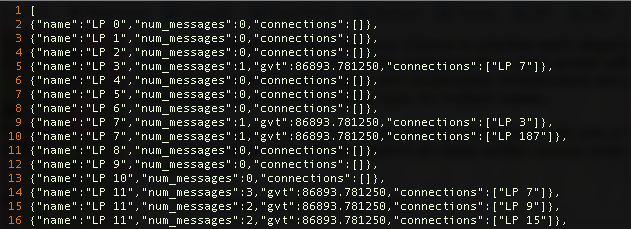
\includegraphics[width=5.0in]{json.png}
\caption{Example of LP connections JSON file created from the raw data.}
\label{json-file}
\end{figure*}


\section{User Interface}
We have developed an interface available on the web using the D3.js~\cite{d3} library as well as the parallel coordinates library built on top of D3 by Kai Chang~\cite{chang}.  It's hosted at https://caitlinross.github.io/ vis-project/src.  In this section, we first describe our original interface plan.  Then we discuss the actual interface and changes we had to make from the original plan.  

\begin{figure*}[!ht]
\centering
   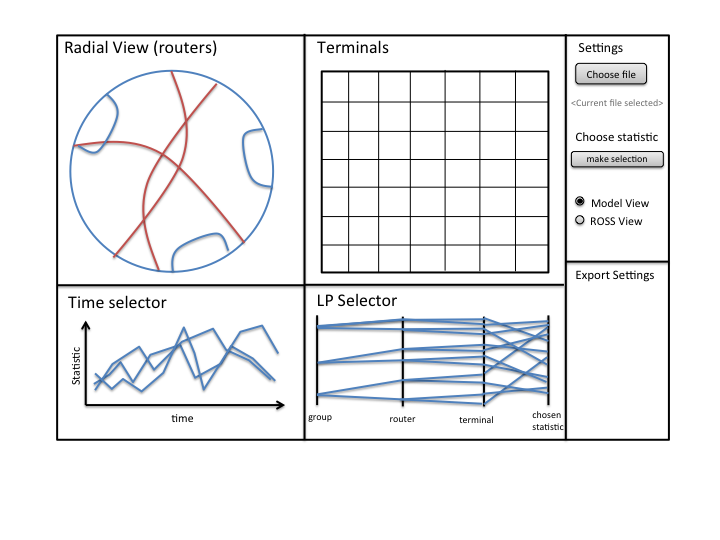
\includegraphics[width=5.0in, clip=true, trim=0 1in 0 0]{../../figures/gui-diagram/Slide1.png}
\caption{Model View}
\label{model-view}
\end{figure*}
\begin{figure*}[t]
\centering
   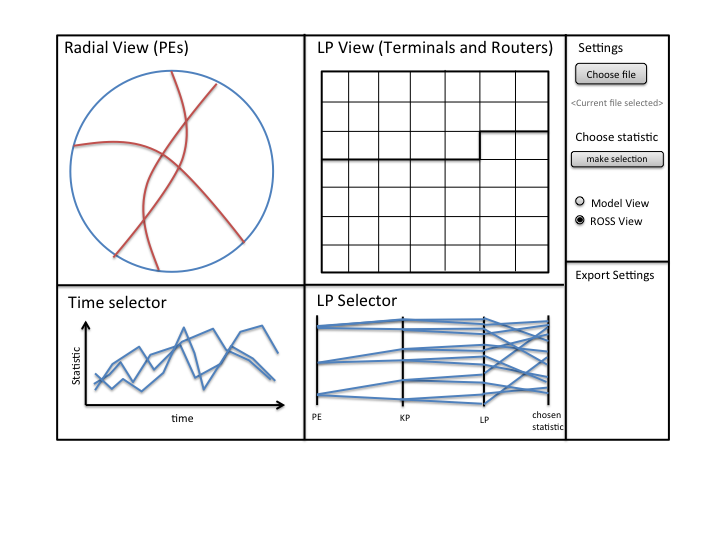
\includegraphics[width=5.0in, clip=true, trim=0 1in 0 0]{../../figures/gui-diagram/Slide2.png}
\caption{ROSS View}
\label{ross-view}
\end{figure*}
\subsection{Original Plan}
We planned for our interface to have two main views: a Model View (Figure \ref{model-view}) and a ROSS View (Figure \ref{ross-view}).  For both views, there is a settings area on the right side of the screen.  Here a file can be selected to load in the data.  You can also choose from a drop down box which statistic to view data for.  Then the user can select either of the two views.  Below that is an export settings area. Original plans for this space was to allow the user to export the entire workspace (i.e., all four graphs) as an image as well as the ability to save each graph as its own image file.  

The workspace of the GUI contains four different interactive visualizations that change depending on whether the Model View or the ROSS View is chosen.  This part of the interface was inspired by Cheng et al.~\cite{cheng}. For the Model View, which is shown in Figure~\ref{model-view}, we have a radial diagram in the upper left corner of the workspace.  This will have routers placed on the circle, with edges representing the links between routers.  Currently the red edges show global connections among the routers, while the blue edges show local connections.  For the actual interface, we have two ideas we are considering for the edge colors.  One way is to keep the different colors for the two different connections and vary the saturation of the color based on the values of the statistic being measured.  The other way is to use the same sequential color scheme for both types of links.  In the ROSS view, shown in Figure~\ref{ross-view}, the PEs will be placed on the circle, with connections between PEs representing the communication between PEs during simulation.  Based on the mappings of LPs to PEs in both network models, it is possible for any PE to communicate with all other PEs, but we will use a similar color scheme as what is used in the Model View.  Particularly for large-scale runs (for either the ROSS or Model views), we will probably need to use hierarchical edge bundling~\cite{jia} in order to make the diagram easier to read and understand.  

The LP selector is shown in the bottom right of the workspace area.  This is a parallel coordinates graph.  For the Model View, the axes are for groups, routers, terminals, and the chosen statistic.  For the ROSS view, the axes are PEs, KPs, LPs, and the chosen statistic.  We are also considering having additional axes shown for all statistics that are being measured, in order to provide additional context.  Brushing~\cite{hauser} can be used on the axes to select a subset of the data, which will also update the routers/PEs being shown in the radial view.  

We will also have a time selector, shown in the bottom left corner of the workspace, although we are currently planning to use line graphs instead of streamgraphs used in~\cite{cheng}.  The statistic being viewed can be selected in settings and will contain data for all of the LPs.  This graph should look similar for both the Model and ROSS views.  The data shown on this graph can also be updated based on the choices made in the LP Selector graph. Also, this time selector graph will allow the user to select specific time periods of the simulation to focus in on any anomalies or interesting time periods. After selecting a time period, the information in all three other graphs will adjust according to the data within the new time period. 

Finally, we have a fourth visualization, which is placed in the upper right corner of the workspace.  This allows for viewing some aspects of the data in more detail.  In the Model View, this is a grid of terminals that are connected to the routers.  The terminals will be colored as a heat map based on the values of the statistic being viewed. For example, if the statistic selected is remote events, then each block representing a terminal will be rendered with a cool color if that termal has little remote events and a hot color if it has many remote events. Also, when one or more routers are selected in either the radial or parallel coordinates views, the corresponding terminals connected to those routers will be highlighted in this grid view using a thicker boarder. For the ROSS View, squares in the grid can represent either terminals or routers, which will be separated by a thicker border (as seen in Figure~\ref{ross-view}).  The terminals and/or routers shown here can be updated by all of the previously described visualizations in order to be able to view only certain entities.  
\begin{figure*}[t]
\centering
   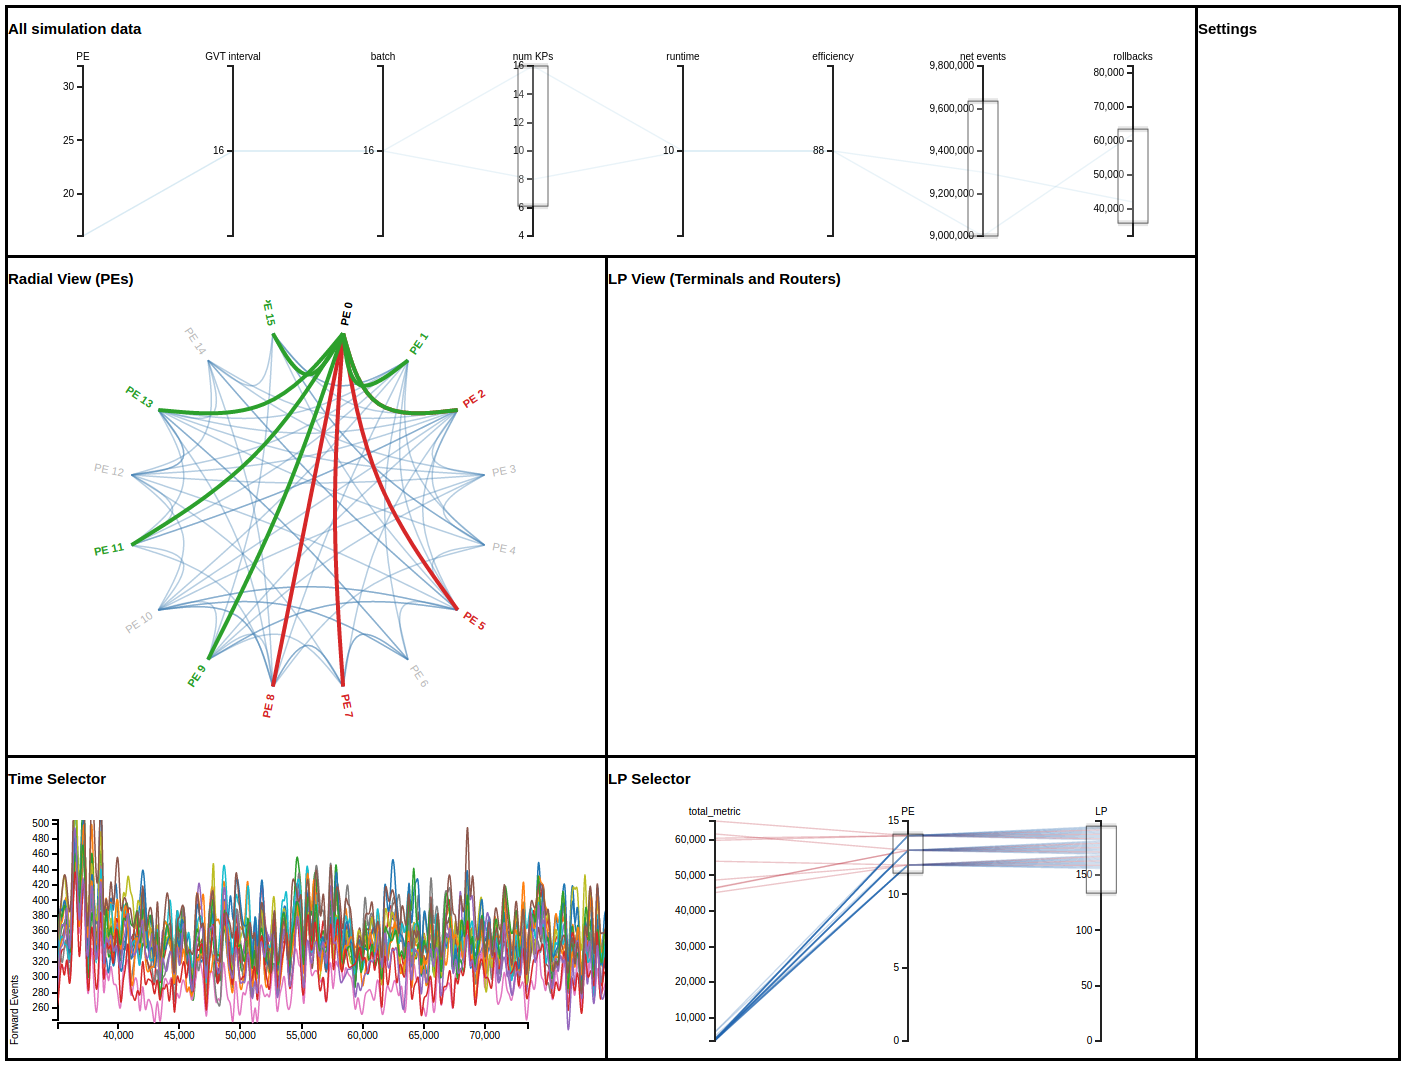
\includegraphics[width=6.5in]{demo1.png}
\caption{In progress visualization used for in-class one-on-one demonstrations}
\label{intm-vis}
\end{figure*}

\subsection{Intermediate Progress}
% from progress report 2
A week or so into the project implementation, we decided to make a change to the layout. At the time, we didn't find the original LP view grid design to be effective in portraying our event based simulation data. As seen in Figure \ref{ross-view} showing the original interface, we planned to create a grid showing the LPs that would be a heat map based on the values of whatever metric being viewed. After some browsing on the D3 examples page, we came across the following visual layout https://github.com/marmelab/EventDrops, which shows zoom-able event based data over time for many entities. We wanted to modify this so that each row is an LP belonging to the selected PE (processing element).  Simulated time would replace the actual time in the example.  Then we could zoom in and out on the simulated time and see where events fall over time. 

Unfortunately, this new example layout didn't come with much documentation and we couldn't get it implemented in time for the one-on-one in-class demonstrations. Instead, we had to leave the LP view empty for the demos as seen in Figure \ref{intm-vis}. Moving forward, we ended up making the final decision to replicate the layout shown in the left radial PE view for the LPs as well. The radial view allows us to not only show event intensity but also communication links between LPs.

\begin{figure*}[t]
\centering
   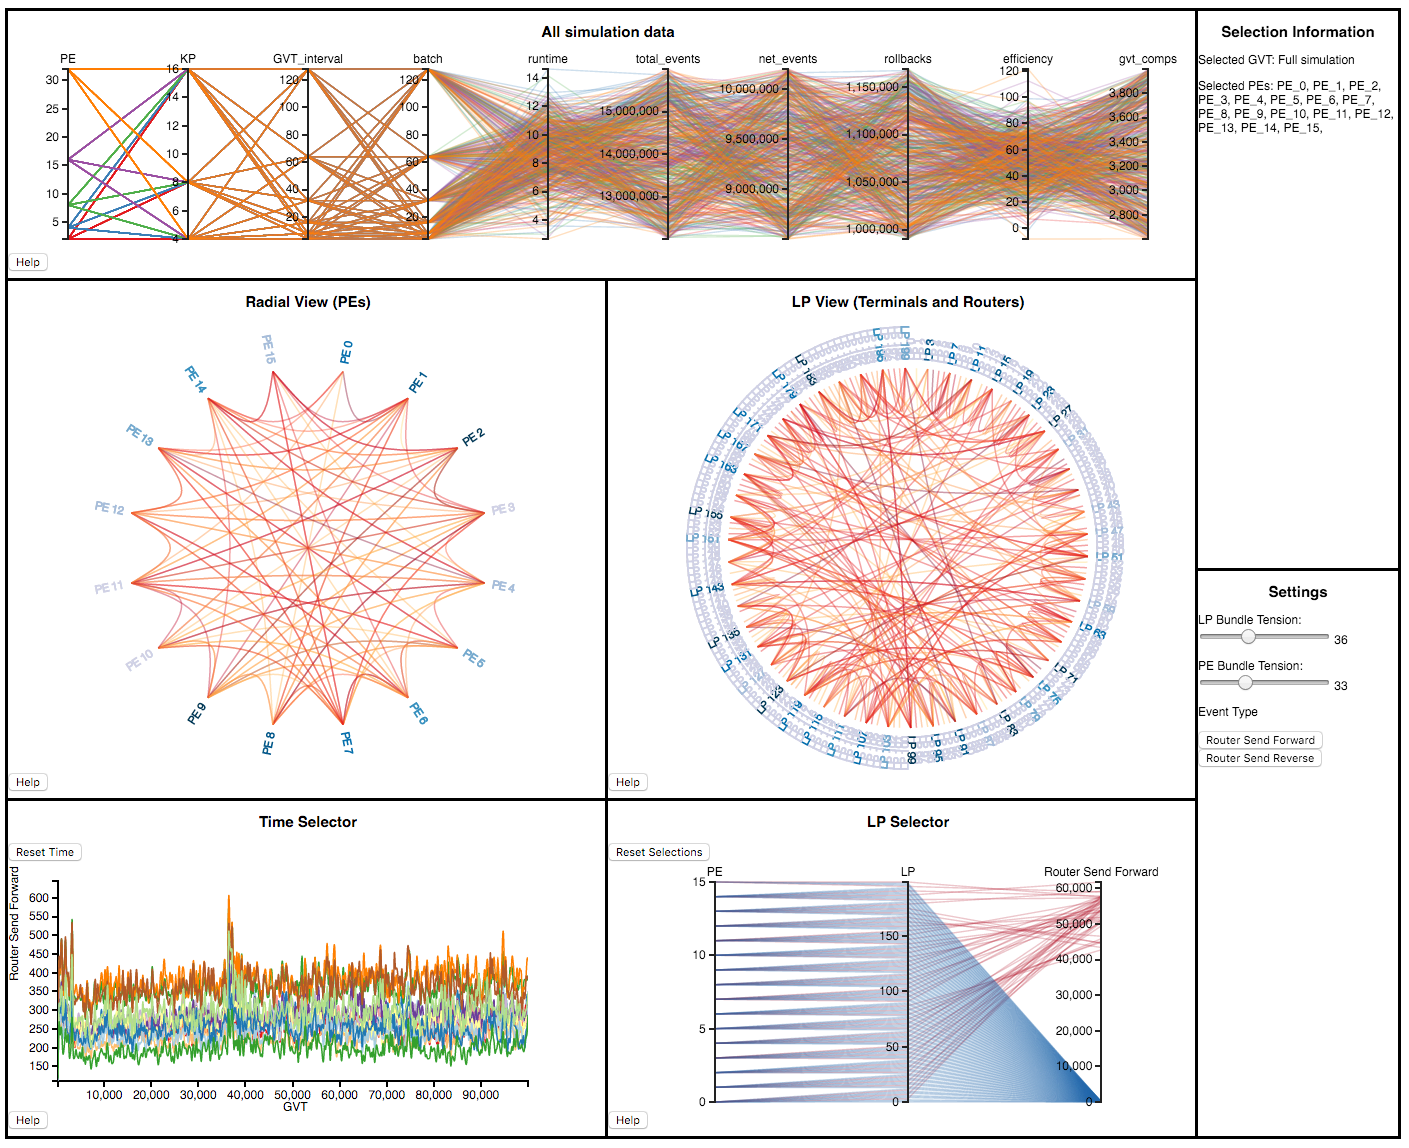
\includegraphics[width=6.5in]{actual-vis.png}
\caption{Full Visualization Interface}
\label{actual-vis}
\end{figure*}

\subsection{Actual Visualization}
Our final visualization interface is shown in Figure \ref{actual-vis}.  This section describes the layout and functionality, as well as changes made from our original plan.  We realized that our original plans were very ambitious for a short-term project, so we decided to focus on only the ROSS view described previously (instead of the Model View).  In the future, we can extend this to integrate model-level statistics.  

\begin{figure*}[t]
\centering
   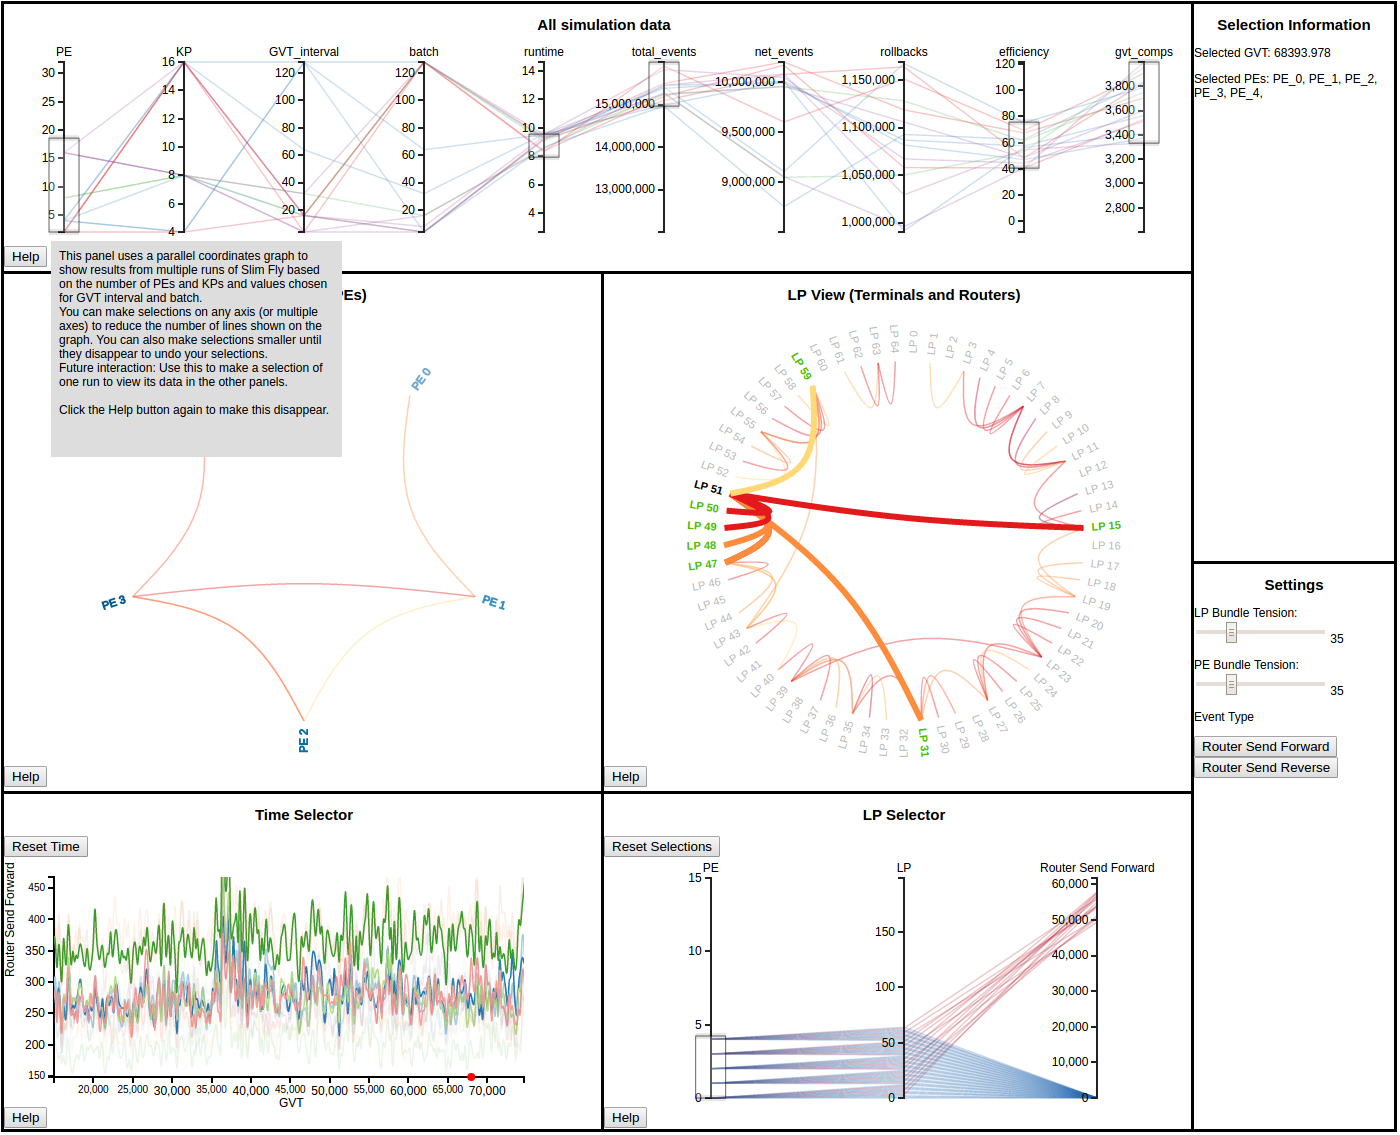
\includegraphics[width=6.5in]{Interactive.png}
\caption{Full Visualization Interface Depicting Interactions}
\label{interact-vis}
\end{figure*}

The first problem we noticed with our visualization is that it would be really tedious to have to manually select and load data for each simulation run.  Because of the different number of simulation parameters that can be changed, this can result in many different runs being made.  This large number of runs presents us with another higher-level data selection layer that we hadn't initially taken into account.  In response to this, we have decided to generate another parallel coordinates graph at the top of the visualization layout. This parallel coordinates graph will present the high-level results such as runtime and efficiency for all simulation runs and allow the user to select one run. Currently, this is showing randomly generated data, since we decided to focus on only one slim fly run.  In the future, we will update this with actual simulation data and allow the user to select one or more runs to look at the simulation specific event data. After selection, the  detailed event-based results for that run will be displayed in the other four panels.

\subsubsection{PE View}
In this view, the main goal is to give visual insight into the distribution of messages being generated and transferred between processing elements (PEs) in the simulation. At large scale, this distribution plays a very large part in how well the simulation will perform and is very hard to understand with a simple efficiency number. 

Very similar to how it was originally designed, each PE is represented by a corresponding text label and is colored based on the intesity of the selected metric for that PE. For example, if we are looking at forward message sends, then a given PE will have a dark color if it has a large number in respect to the other PEs. In the case of very few forward message sends, the PE will have a very light color. The color palette for the PE radial view is a sequential single tone blue for simplicity and is selected using colorbrewer2 \cite{brewer}. The links between PEs are also colored in a similar approach. Links with many events of the selected type have a darker color than links with less events. This time the color palette is a sequential multi hue red that has been chosen because it gives the best distinction between the thin lines. Again, the color palette was selected using colorbrewer2.

Various levels of interaction are also available in the PE radial view. As shown in the LP view in Figure \ref{interact-vis}, when hovering the mouse over any label in the graph, the connections corresponding to that PE are highlighted as are the labels at the end of the connections. When making selections of PEs in the LP selector view, the radial PE view is updated accordingly to show only the connections and activity for the selected PEs. This functionality is shown in the PE view in Figure \ref{interact-vis}. Finally there are also tool tips (which are located in each view) that describe the functionality and interaction of the view.

\subsubsection{LP View}
The LP view first came about when thinking of an approach to visualize the many complex interconnections of LPs in the simulation. Similar to the interaction of PEs, visualizing the interaction of LPs provides insight into how well a given routing algorithm is performing under a certain workload. Hot spots are very hard to detect via text output but very easy with visualization. 

As previously mentioned, major changes have been made throughout the implementation of the LP view. We started off wanting to use a grid structure to layout all LPs in the simulation and use a heat map coloring scheme to indicate the intensity of the selected simulation metric per LP. We quickly found that this approach wasn't the most effective as it left out the connection and link information between LPs. Finally, we ended up going with another radial diagram with the same coloring scheme as is done in the PE view. Each LP is represented by a corresponding text label and has lines connecting the LP to all connected LPs in the simulation. The same heat map coloring is applied as is done in the PE view. 

The interaction is also very similar to the PE radial view. Hovering on a label in the graph highlights it's corresponding connections. Also, making LP selections in the LP selector view adjusts the LPs shown in the LP radial view. This allows focussing attention on subsets of LPs to further investigate hot spots, verify connections and analyse event distribution.

\subsubsection{Time Selector}
The time selector was developed as originally planned, except we decided to group the LPs by their PEs.  Since there are 200 LPs, it was difficult to read.  Even with 16 PEs in the data set we used, it is still difficult to see all of the lines at once.  However, you can see peaks in the graphs and use that to determine what GVT you want to look at.  You can click on the x-axis to make your GVT selection.  A red dot will be placed on that point and the selected GVT will be shown in the Selection Information Panel on the right.  We wanted to make the time selection update both radial views, but we ran out of time to fully implement that feature.  The time selector also allows the user to zoom in and out as well as pan across the graph.  To allow this feature to work smoothly, we had to bin the data for the individual GVTs into 500 bins.  At the top of the graph there is a reset button that allows the user to view the full simulation again.

\subsubsection{LP Selector}
The LP selector is also similar to the original plan, except that we do not show the kernel processes (KP) that each LP is assigned to.  The component allows the user to make selections on any subset of the axes to choose which specific LPs and PEs they want to view data for.  This updates the Time Selector Panel by lowering the opacity of the lines for any PE that is not selected.  This also updates which PEs and LPs are shown in each of the radial views.  It works well for the PE view, however there is some issue with the LP view and it only works if LP\_0 and PE\_0 are chosen.  This component also contains a reset button that allows all of the LP/PE selections to be easily undone.  

\subsubsection{Selection Information}
The Selection Information Panel currently shows the selected GVT (or specifies the Full Simulation if no time has been chosen).  It also shows the list of PEs that have been selected.  We considered adding the list of LPs, but this probably would not be useful, especially as simulations scale up in the number of LPs.  An idea for some other potentially useful information we  display here could be the top 5 busiest links.

\subsubsection{Settings}
The Settings panel currently has slider bars that allows the user to change the bundle tension for each radial view.  There are also buttons that allow you to toggle which metric you want to view.  Currently we have only the forward and reverse events for router LP sends enabled.  Next we plan to enable viewing of the other event types collected.  We may also convert this to using check boxes, so that the user can combine results for different event types.  For example, if the user wants to see how the status of the full simulation for all forward events regardless of type, the user could select all of the forward event types (i.e., router sends, terminal sends).  

\section{Timeline}
Our original timeline for this project is as follows:
\begin{itemize}
\item Finish development of the ROSS statistics collection
\item Perform runs of network models with statistics collection enabled
\item Create the GUI, focusing first on the radial view and the LP selector
\item Add the time selector and Terminal/Router grid
\item Integrate all views to perform automatic updates upon selection changes in any one view
\item Solicit feedback from advisor on the level of interaction and insight available in the visualization
\item Implement/adjust/revise implementation based on the analysis in the previous step
\item Finalize report and presentation
\end{itemize}

As previously described our data collection method changed several times over the course of the project.  After the first time, we decided to only do one specific simulation run and focus on that until we could be sure that our data collection wouldn't change.  We were able to create all of the visualization views we wanted, as well as incorporate most of the interaction between components.    Our next step is to finish fixing these final pieces (e.g., GVT selection updating the radial views) and then we will look for feedback from our advisor and research group.  

\section{Risks and Limitations}
One of our anticipated risks was being unable to collect the data we needed.  This ended up not being much of an issue as we eventually decided to focus on a smaller model and single run.  Our other anticipated risk was that neither one of us is particularly experienced with Javascript and we've had some difficulty with certain features of D3 on previous assignments.   The development of some aspects of our interface definitely ate up more time than we would have liked, but we were still able to complete most of the features we planned on.  

A potential limitation of our work that was brought up by some students in our presentation feedback is that the interface may be too busy.  This is a valid concern, but we believe that each component shows a unique look into the data set and that because these aspects are all linked, they should be shown together on one window. 
    

\section{Feedback from other students}
During the in-class one-on-one demonstrations, we received a large number of beneficial comments and questions. These comments and questions allowed us to take a step back and see how the visualization looked from the eyes of a potential end user and non-developer. Most of the comments were slight layout fixes that we were easily able to incorporate, making for a much cleaner and efficient presentation. Unfortunately, none of the people we were able to give a demonstration to fall under our "ideal" audience as none of them have the required background in discrete event simulation. However, some had heard about our simulation back-end and with a quick crash course felt they had a decent understanding of the information being presented. In the future we will be releasing the visualization to our research group to get a better sense of how well the visual tools we provide, capture and explain the data generated in the simulations. Since this is a first proof of concept, we foresee this visual tool evolving over time in an iterative manner as end users get familiar with the interactions and ask for more features. The following is a list of common comments and questions we received from "demoers" that we were able to take into consideration and address by the end of the project. 

\begin{itemize}
\item Add Radial bundle tension selection to the "Settings" panel
\item Will there be a legend with the information?
\item Add a description to each plot to describe the available interactions (pop up bubbles) and how to use the figures
\item Make the lines thicker in the top parallel coordinates graph
\item Make font larger on axis labels
\item What questions is such a visualization going to answer?
\item Is there a way to unselect?
\item Change saturation of PE links (radial view) based on value of the metric
\end{itemize}

The following list consists of the comments and questions we were not able to address.

\begin{itemize}
\item How will the visualization perform with large amounts of data?
\item Is there any desire to perform the visualization in-situ?
\end{itemize}

Since we had multiple visualizations we wanted to get up and running and interacting with one another, we decided to focus on the smallest model possible. Much of the work we performed was proof of concept so we have yet to do perform scaling analysis to see if the visualization becomes non-responsive with much large models and corresponding datasets. Also, as mentioned before, if we are able to iron out all the details in the visualizations then we would like to look into in-situ visualization to give developers the unique opportunity to understand their simulation as it runs. 

\section{Prior Work}
This work is an extension to projects both authors are currently involved with. Caitlin is actively involved with the ROSS discrete-event simulation framework but her work involves development of a model separate from the Slim Fly and Dragonfly network connections. Noah is also involved with ROSS and is the developer behind the Slim Fly network model. Everything done in this course project has been a large extension of prior work. Such complex data collection hasn't been performed in ROSS before and neither has any sort of visualization of that data been done. 

\section{Related Work}
A previously mentioned, a large part of our visualization interface was inspired by Cheng et al.~\cite{cheng}.  In their paper, they describe an interactive interface that visualizes only the network traffic over a 5D torus network and not the traffic/interaction of the underlying simulation system.  They have a radial diagram that shows network traffic, a parallel coordinates graph to allow for node selection, and a stream graph which shows some property of the network over time as a streamgraph.  The streamgraph also allows the user to select a point in time which updates the view in the radial diagram.  Similarly nodes can be selected in the parallel coordinates to update the radial diagram.

Similar to our work, Bhatele et al. \cite{DragonVis} has used radial graphs to visualize simulated large scale HPC dragonfly network activity. They use the radial graphs to show how multiple applications running on a supercomputing system can be affected by the interconnection network. Our work however is focusing on one application running at scale. Also, unlike our work which simply uses a label with dynamic color intensity based on the selected metric, the Bhatele et al. approach adds a group of dynamic color intensity dots to show each individual processor in the system. 

\section{Debugging Visualization}

\begin{figure*}[!ht]
     \centering
%     \subfloat[][dot plain]{\epsfig{file=class-net/class-net-Datastructures-dot.png, height=1.5in, width=1.80in}\label{vis-50-0}}
%     \subfloat[][circo plain]{\epsfig{file=class-net/class-net-Datastructures-circo.png, height=1.5in, width=1.80in}\label{vis-90-0}}
%     \subfloat[][neato plain]{\epsfig{file=class-net/class-net-Datastructures-neato.png, height=1.5in, width=1.80in}\label{vis-95-0}}
%     \subfloat[][osage plain]{\epsfig{file=class-net/class-net-Datastructures-osage.png, height=1.5in, width=1.80in}\label{vis-100-0}}\\
     \subfloat[][Terminal LP 20 Connections]{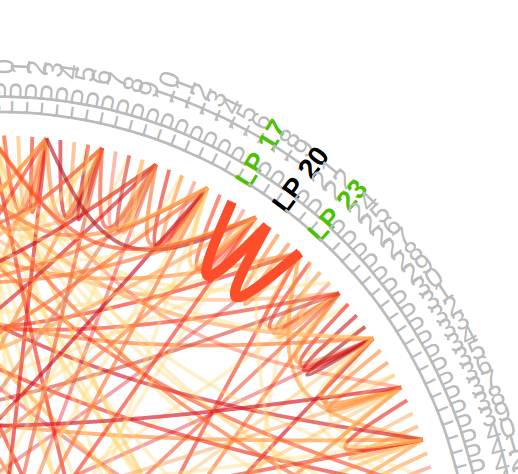
\epsfig{file=debug1.png, height=3.0in, width=3.0in}\label{debug1}}
     \subfloat[][Router LP 23 Connections]{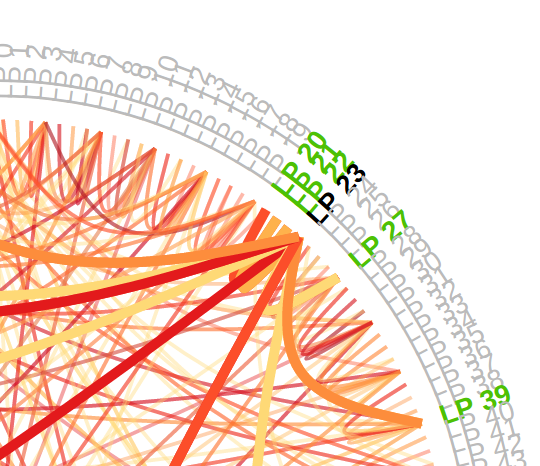
\epsfig{file=debug2.png, height=3.0in, width=3.0in}\label{debug2}}\\
%     \subfloat[][osage]{\epsfig{file=class-net/class-net-Datastructures-weight-osage.png, height=1.8in, width=2.80in}\label{vis-100-1}}\\
          \caption{Visualizations showing the debugging capabilities. Figure \ref{debug1} shows terminal LP 20 has more than one connection, which isn't possible. It's only connection should be to router LP 23 shown in Figure \ref{debug2}. }
     \label{debug}
\end{figure*}

After having collected and visualized data in the radial LP view, we noticed a major issue. As seen in Figure \ref{debug}, the radial view showed us that some of the terminals had more than one connection in the network of LPs. Of course, this shouldn't be happening as all terminals are only connected to exactly one router which relays messages throughout the network to their destination terminal. At first glance, it appeared to be a bug in the simulation (the simulation which had recently generated results that were published), which caused some anxiety. After further investigation, the visualization showed the extra connection was a consistent offset which led us to the data processing where we found and fixed the bug. Not only does the radial view prove that our data processing and visualization algorithms are correct but also that the original simulator is indeed correct. This tool makes it very easy to verify connections as it is much easier to do so visually than scanning line by line through text files.

%%%%%%%%%%%%%%%%%%%%%%%%%%%%%%%%%%%%%%%%%%%%%
%% From progress report 3
%%%%%%%%%%%%%%%%%%%%%%%%%%%%%%%%%%%%%%%%%%%%%
\section{Potential User Study}
Since the content of our visualization is geared towards a very specific field of research, the user study for our visualization would need to separately test the effectiveness of the interactions and the effectiveness of understanding the data. In order to understand the data, the user will need to either have a background in discrete-event simulations or be willing to sit down for a 15 minute tutorial/lesson on the subject. Those that do not have the necessary background and don't do the tutorial/lesson will only be able to test out the effectiveness of the interactions and data selections. Those with the necessary background can also be tested on how well the visualization conveys the data and how much new insight the visualization provides.

The "un-knowledgeable" group of users would be asked to complete a number of tasks requiring the user to interact with the visualizations to select data. Our visualization has multiple windows presenting different sets of interconnected data and it's important for users to understand the connections between the different windows. The specific tasks would be along the following:
\begin{itemize}
  \item Select the simulation with the longest runtime. 
  \item Select PEs (processing elements) 2-27,  LPs (logical processes) 40-45, time slice 67 and tell me which LP has the largest number of message sends.
\end{itemize}
  
For the second group of "knowledgeable" users, we would prefer if they could bring their own data set to see how much new insight can be uncovered but we can also provide our own. These users would be subjected to the same interactive tasks as the "un-knowledgeable" users and in addition, they would be asked a set of qualitative questions that determine if the user is able to easily answer questions that would require copious amounts of time digging through data to answer with out a visualization.
\begin{itemize}
\item Why is the slowest running simulation running so slow?
\item In the run with 256 nodes, why is one node sending so many more messages than it's neighbors?
\end{itemize}

\section{Division of Work}
We each worked at least a little bit on all aspects of the project.  Caitlin planned out some working designs and then discussed it with Noah to make edits until we settled on our proposal design.  Since the Slim Fly model was developed by Noah, he set up the data collection (both adding code and performing the runs).  While Noah set up the data collection, Caitlin worked on setting up the layout of the components for the interface.  Caitlin created the All Simulation Data, Time Selector, and LP selector views, while Noah worked on the both of the radial views.  We both did debugging of the post-processing program once we discovered issues with our data.  We also both worked on the various interactive features linking the individual components.  We both worked on the initial proposal writeup as well as this final report and we took turns working on the progress reports.  We both worked on the presentation slides.  


%\section{Conclusions}

%\end{document}  % This is where a 'short' article might terminate

%ACKNOWLEDGMENTS are optional
%\section{Acknowledgments}

%
% The following two commands are all you need in the
% initial runs of your .tex file to
% produce the bibliography for the citations in your paper.
\bibliographystyle{abbrv}
\bibliography{final}  % sigproc.bib is the name of the Bibliography in this case
% You must have a proper ".bib" file
%  and remember to run:
% latex bibtex latex latex
% to resolve all references
%
% ACM needs 'a single self-contained file'!
%
%APPENDICES are optional
%\balancecolumns


%\balancecolumns % GM June 2007
% That's all folks!
\end{document}
